With the method described in the algorithm \ref{alg:simil_1}, we created a figure where the metrics are presented with increasingly different datasets: figure \ref{fig:lineplot}.
%Then we compared the difference in the metric across iterations, rendering figure \ref{fig:boxplot}.


%TC:ignore
\begin{figure}[htbp]
\centering
\caption{Plot showing the decrease of the metric over increasingly changed datasets. The X axis represents the number of columns mutated. The Y axis represents the value of the metric and the hue represents the algorithm used to calculate the metric.}\label{fig:lineplot} 
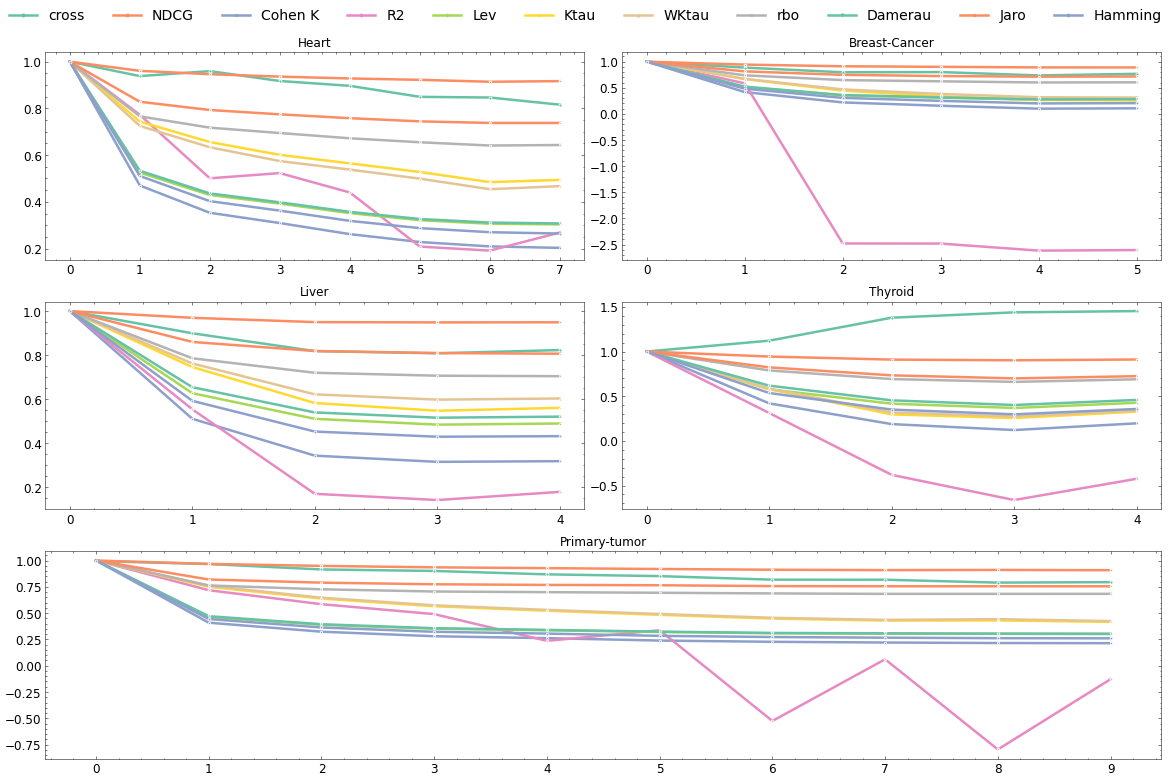
\includegraphics[scale=0.32]{figures/multiple_datasets.png}
\end{figure}
%TC:endignore


%TC:ignore
\begin{figure}[htbp]
\centering
\caption{Plot showing the values at 50\% columns mutated across all datasets and algorithms per metric type}\label{fig:boxplot} 
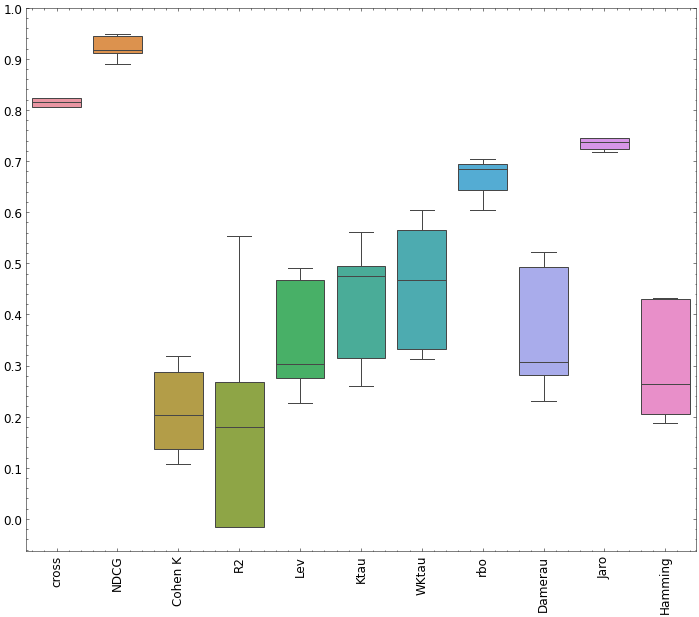
\includegraphics[scale=0.40]{figures/50_percent_data.png}
\end{figure}
%TC:endignore


The number of repetitions and how that impacts the variance of the scores is shown in figure \ref{fig:facet_plot}.






%TC:ignore
\begin{figure}[htbp]
\centering
\caption{Plot the variance of different repetitions for every metric and the number of different columns changed. X is number of columns mutated. Color is number of repetitions for each mutation and Y is the variance of the data. }\label{fig:facet_plot} 
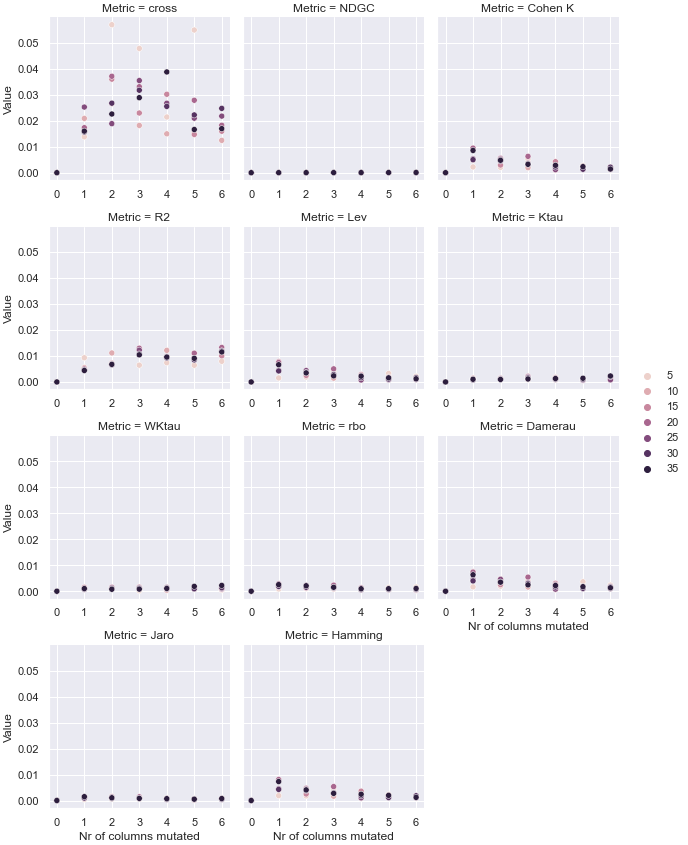
\includegraphics[scale=0.55]{figures/facet_plot.png}
\end{figure}
%TC:endignore

As for the test for the synthetic and real dataset, the results are displayed in figure \ref{fig:synth_result}.
%TC:ignore
\begin{figure}[htbp]
\centering
\caption{Result on a synthetic and real data }\label{fig:synth_result} 
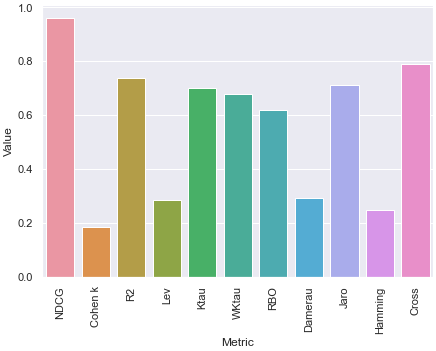
\includegraphics[scale=0.65]{figures/synthetic.png}
\end{figure}
%TC:endignore